\section{Proposed Architecture}
\label{sec:ocpl_architecture}
This section provides the effective implementation of the general modular architecture described in Section \ref{sec:cod_problem}. Since the Command Analysis task being solved is Conditioned-Object Detection (Chapter \ref{ch:cod}), the focus here is on how the COD module is effectively integrated into the control framework.

The COD module is integrated into two different architectures, which vary in the number of control modules they use. Section~\ref{sec:ocpl_architecture_scm} outlines an architecture that employs a single control module to predict actions for the entire trajectory. In contrast, Section~\ref{sec:ocpl_architecture_dcm} describes an architecture that splits the control module into two distinct parts: one for computing actions during the reaching phase, and another for the final phase, where the specific primitive depends on the task.

\subsection{Single control module}
\label{sec:ocpl_architecture_scm}
The architecture (Figure \ref{fig:single_control_module}) composed of a single control module is essentially an instance of the general modular architecture depicted in Figure \ref{fig:end_to_end_vs_modular}. Specifically, the Command Analysis Module is replaced by the CTOD module (Section \ref{sec:cod_tod}), which takes as input the current agent observation $o^a_t$ and the command $c_m$, producing a task embedding represented by the \textit{target-object bounding box}, i.e., $z^{task}_t = bb^{target}_t$.

The Backbone Module, responsible for generating the control embedding $z^{control}_{t}$, is replaced by the same backbone used in MOSAIC. This backbone is a combination of a Convolutional Network, which encodes the agent observation $o^a_t$ and the demonstration frames $c_m$, and a Self-Attention mechanism to create correlated agent and command embeddings (Section \ref{sec:bc}). 

Finally, the Control Module follows the same implementation as in MOSAIC \cite{mandi2022towards_more_generalizable_one_shot}. In this case, the actions generated by the control module are sampled from a multivariate logistic distribution (Equation \ref{equation:logistic_distribution}), where the distribution parameters $\mu_{i}$ and $\sigma_{i}$ are estimated by MLPs implementing the Control Module.

\begin{equation}
    \label{equation:logistic_distribution}
    a_{t} \sim \sum_{i=1}^{m} \alpha(z_t) \, logistic(\mu_{i}(z_t), \sigma_{i}(z_t))
\end{equation}

Here, the embedding $z_t$ is a concatenation of $z^{control}_{t}$, generated by the MOSAIC Backbone, and $bb^{target}_t$, produced by the CTOD Module.

\begin{figure}[t]
    \centering
    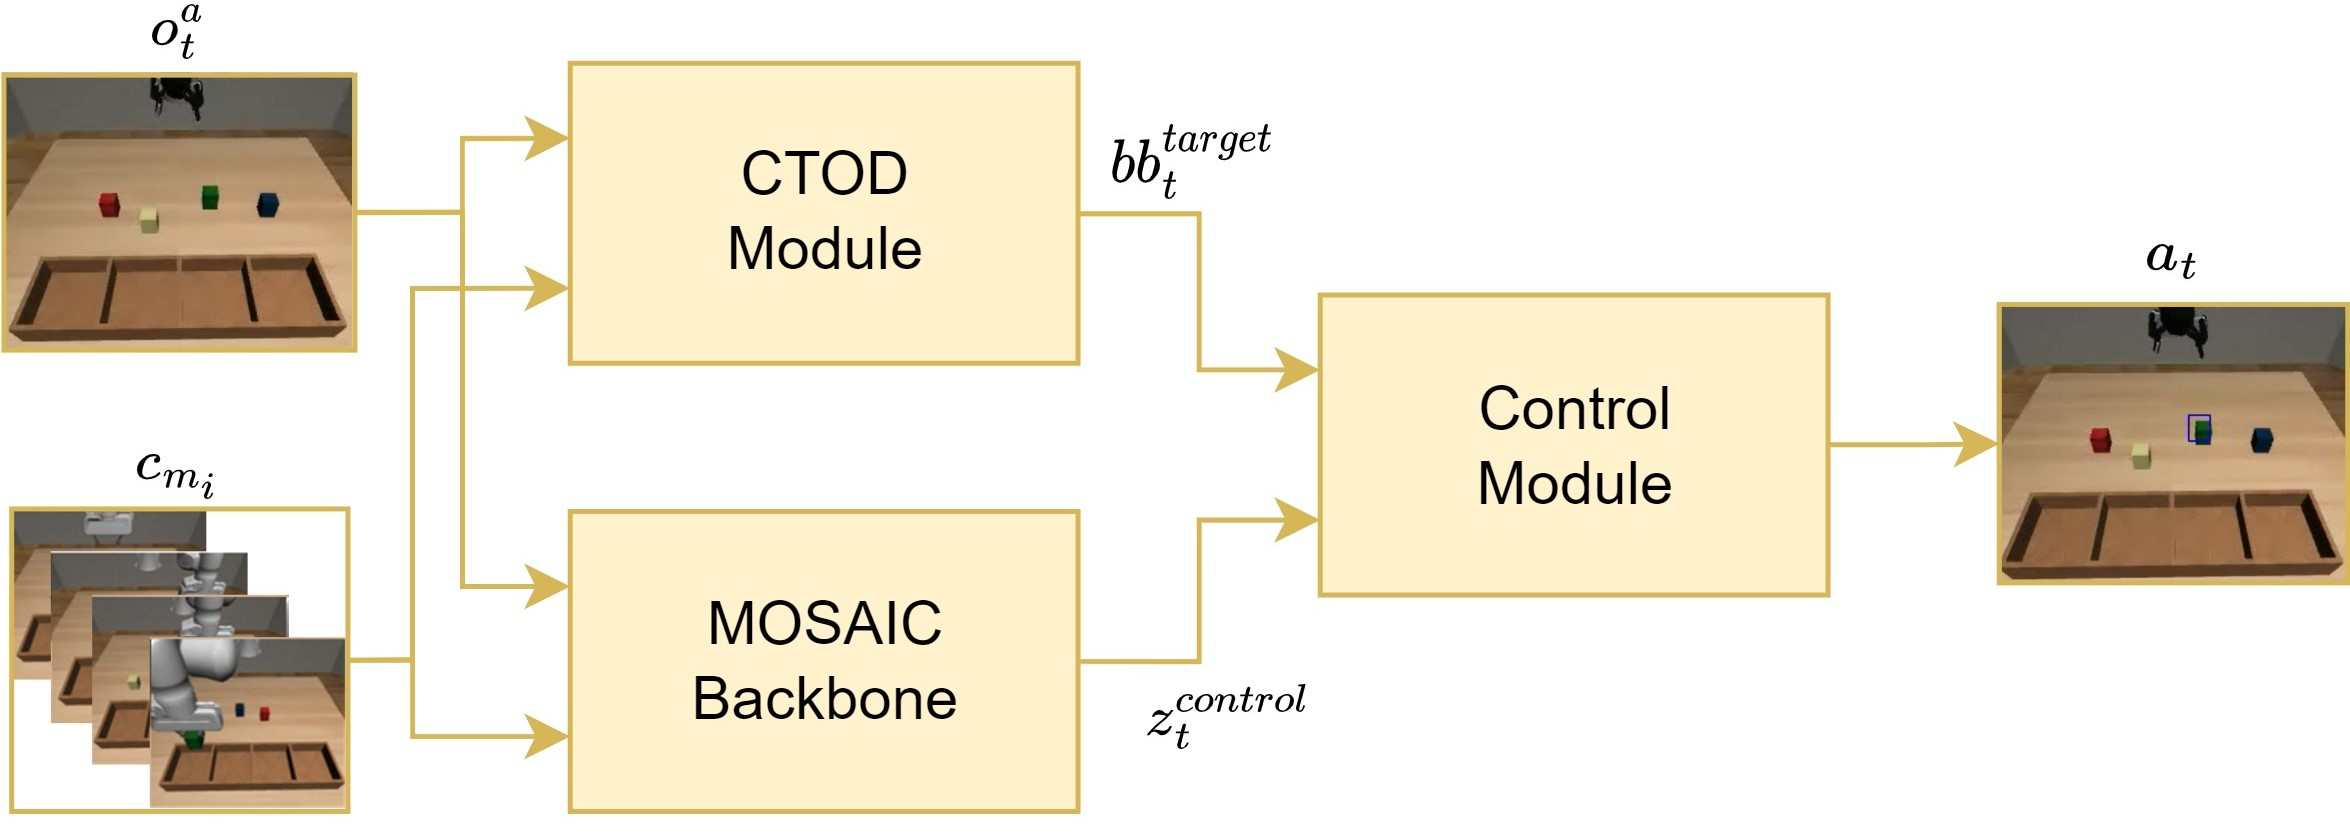
\includegraphics[width=0.9\textwidth]{figures/images/ch3/single_control_module.jpg}
    \caption{Proposed Single-Control Module Architecture. In contrast to the general architecture described in Figure \ref{fig:end_to_end_vs_modular}, the Command Analysis module is replaced by the CTOD module, which generates the bounding box related to the target object. The chosen backbone is the MOSAIC architecture \cite{mandi2022towards_more_generalizable_one_shot}. The control module is now informed by both low-level positional information ($bb^{target}_{t}$) and a control-oriented embedding ($z^{control}_{t}$), enabling it to make more informed decisions.}
    \label{fig:single_control_module}
\end{figure}


\subsection{Double control modules}
\label{sec:ocpl_architecture_dcm}
Regarding the architecture composed of multiple control modules, the discussion must begin with the key observation that the tasks considered can be roughly divided into two phases. The first is generally a \textit{reaching phase}, where the robot must reach a target location. The second phase varies based on the task: placing for Pick-Place, assembly for Nut-Assembly, stacking for Stack-Block, and pushing for Press-Button. Based on this, a dual control module architecture is proposed, with each control module trained to learn the primitive associated with each phase. The rationale behind this approach is that training modules specifically for simpler atomic primitives can result in a more robust and reliable control system.

Figure \ref{fig:double_control_module} illustrates the overall architecture. The main difference can be observed in the bounding boxes received by the control modules. Specifically, the MOSAIC Backbone generates the control embedding $z^{control}_t$, as before. However, the Command Analysis Module, now referred to as the COD Module, generates both the bounding box for the target object, $bb^{target}_t$, and the bounding box for the final placing position, $bb^{place}_t$. 

The $bb^{target}_t$ is provided as input to the \textit{Reaching Control} module, while the $bb^{place}_t$ is supplied to the \textit{Placing Control} module. 

Additionally, each control module operates based on an enabling signal $s^{en}$, which is set to 1 at the beginning of the rollout and remains active until the Reaching Control module generates its first prediction for the closing command. After this point, $s^{en}$ is set to 0, and control is transferred to the Placing Control module.    
\begin{figure}[t]
    \centering
    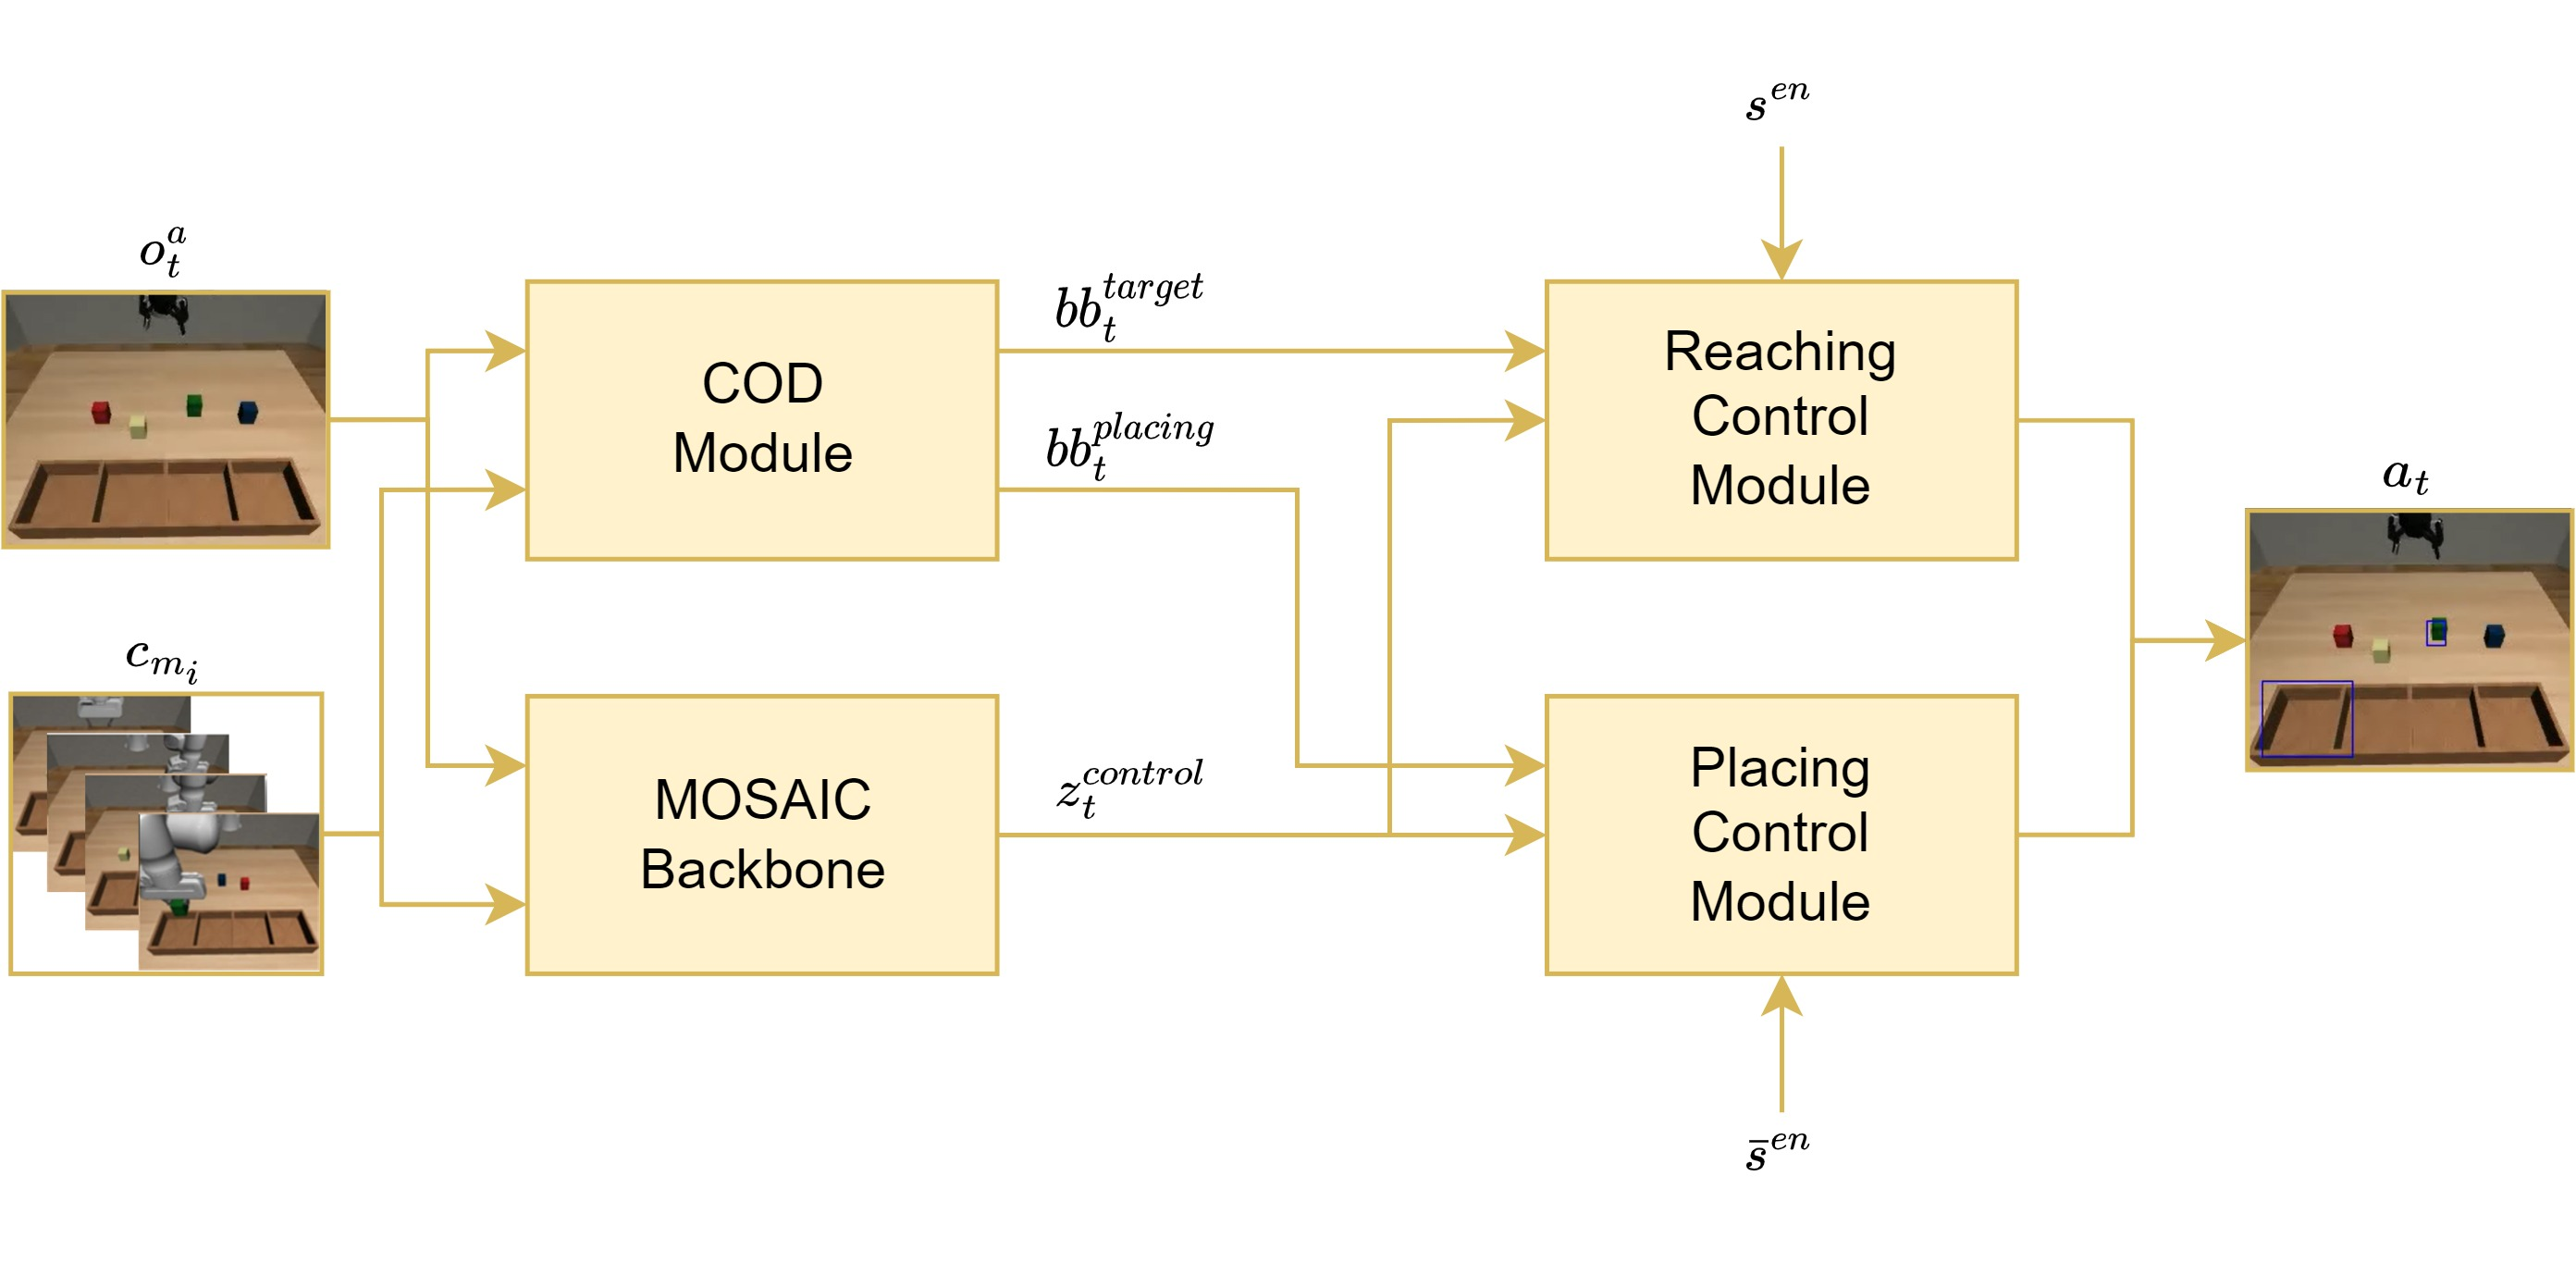
\includegraphics[width=0.9\textwidth]{figures/images/ch3/double_control_module.jpg}
    \caption{Proposed Double-Control Module Architecture. In this architecture, the Control Module is split into two distinct modules, each responsible for learning a specific primitive: the \textit{reaching} primitive and the \textit{placing} primitive. The first module takes as input the bounding box corresponding to the target object ($bb^{target}_{t}$), while the second module receives the bounding box related to the final placing location ($bb^{placing}_{t}$). This separation allows for specialized control during both the reaching and placing phases.}
    \label{fig:double_control_module}
\end{figure}

% \smalltodo{add figure}